\begin{figure*}[t]
    \centering
    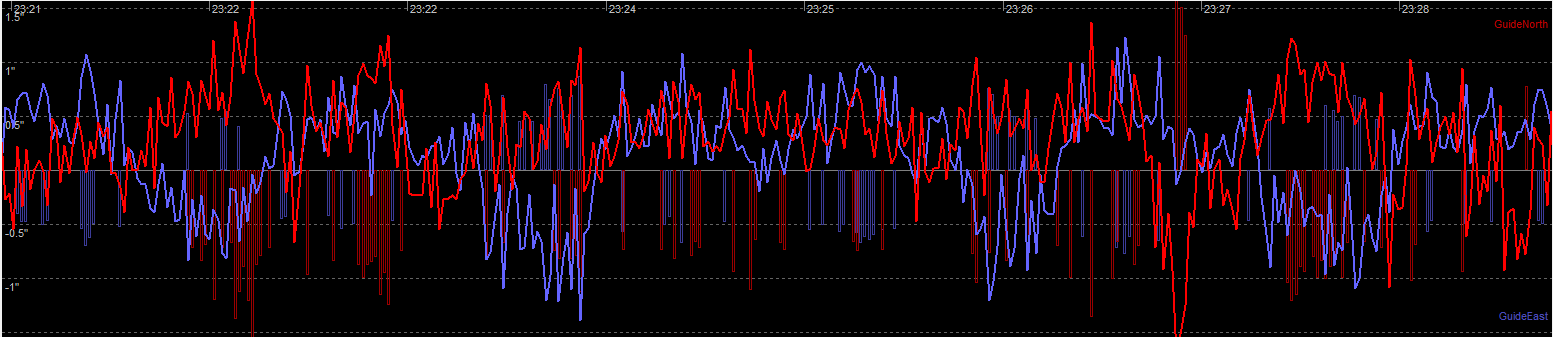
\includegraphics[scale=0.45]{analysis/PHD2/2021-12-09/guide-11-arcsec.png}
    \caption{DEC V1 test: PHD2 log view using arcseconds as units. In pixel the scale is in the range \([-0.4,0.4]\). The sky seeing was \(0.98''\).}
    \label{fig:guide-11-arcsec}
\end{figure*}
\begin{figure*}[t]
    \centering
    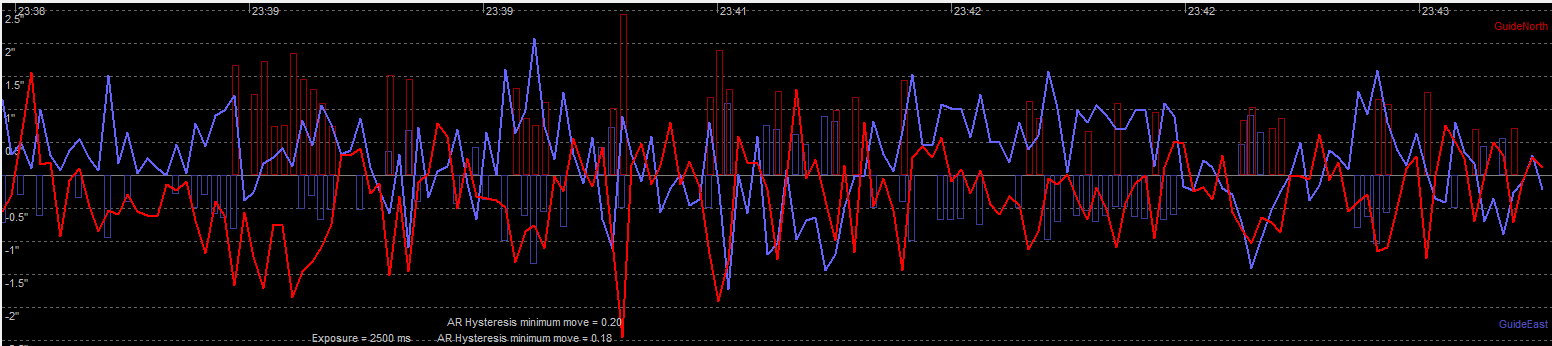
\includegraphics[scale=0.45]{analysis/PHD2/2021-12-23/guide-7-arcsec.png}
    \caption{DEC V1+ test: PHD2 log view using arcseconds as units. In pixel the scale is in the range \([-0.5, 0.75]\). The sky seeing was \(1.80''\).}
    \label{fig:guide-7-arcseconds}
\end{figure*}

\section{Tests}
\label{sec:tests}
% Sidereal tracking is done by the OnStep software, of course.
% Otherwise, since the polar alignment may not be perfect we have decided to equip the telescope with an auto-guiding system controlled by the PHD2 app.
% This, in our mind, should optimize the tracking and permits long-exposure photography which is necessary for optimal results.

% Although separated by the previously mechanization, this auto-guiding system interacts with the mount using ASCOM OnStep telescope drivers, and provide corrections to the tracking.

The test are aimed to estimate the precision of the mount.
Of particular interest are the test using PHD2 which measure the precision in micro-adjustments for the auto-guiding system.

The application used to study the PHD2 plots is the PHD2LogViewer app.
The latter can upload all the guiding session you make, since every session is stored in the PHD2 folder.
The app also make raw statistical analysis which are good parameters to think about.
The root-mean-square (RMS) describe the spread of the data points around some average peak value (like standard deviation).
The value of RMS should be 1 arcsecond or lower for a good guiding.

Before describing the tests, let us show the tracking system, which is composed of a guidescope and a tracking camera.

\subsection{Telescope guidescope}
On the telescope is fixed a 240mm focal length guidescope Svbony SV106.

\subsection{Guidescope camera}
The camera is an old red webcam inserted into the guidescope using an adpter.\footnote{See this useful tutorial \url{https://telescopeguides.com/how-to-use-a-webcam-with-a-telescope/}.}
The result is pretty weird, but it works!
Just look at the following sections PHD2 logs!

\subsection{DEC V1 test}
The DEC V1 has been developed to reduce the mechanism backlash using the idea \textit{the less the number of belts gets, the better the guiding is}.
The resolution power of the mount is reported in table \ref{tab:resolution-power-DEC-V3}.
The extrapolated statistics is reported in table \ref{tab:DEC-V3-statistics}.
\\
\\
\begin{minipage}
    {.5\textwidth}
    \begin{tabular}{c|c|c}
        \hline
        \textbf{Mechanism} & \textbf{microsteps (x360$^{\circ}$)} &\textbf{estimated resolution ('')}\\
        \hline
        RA  & 19200 & 0.21\\ 
        DEC & 12800 & 0.65\\
        \hline
    \end{tabular}
    \captionof{table}{Resolution power using the DEC V1 mechanism. Microsteps is intended as the total number of microsteps around the entire circumference.}
    \label{tab:resolution-power-DEC-V3}
\end{minipage}
\\
After the calibration, we have pointed the Rosetta nebula and start tracking.
The result can be seen in figure \ref{fig:guide-11-arcsec}.
The sky condition was very nice that night with a seeing of \(0.98''\).
\\
\begin{minipage}{.4\textwidth}
    \centering
    \begin{tabular}{ccc}
        \textbf{Statistics}&RMS&Peak\\
        \hline
        RA& 0.47" (0.15 px)& 1.87" ( 0.58 px)\\
        DEC& 0.90" (0.28 px)&-8.12" (-2.52 px)\\
        Total& 1.02" (0.32 px)&\\
        \hline
        \\
        \textbf{Drift}& ("/min) & (px/min)\\
        \hline
        RA& +3.01"/min& +0.94 px/min\\
        Dec& +2.14"/min& +0.66 px/min\\
        Polar Alignment Error& 8.7'&\\
        \hline
    \end{tabular}
    \captionof{table}{DEC V1 test: statistics of the guiding of figure \ref{fig:guide-11-arcsec}.}
    \label{tab:DEC-V3-statistics}
\end{minipage}

\subsection{DEC V1+ test}
We have updated the DEC V1 mechanism to DEC V1+ to introduce a more gear reduction and the possibility to decouple the telescope movement from the gear to perfectly balance it.
The resolution power of the mount is reported in table \ref{tab:resolution-power-DEC-V1p}.
The extrapolated statistics is reported in table \ref{tab:DEC-V1p-statistics}.
\\
\begin{minipage}
    {.5\textwidth}
    \begin{tabular}{ccc}
        \textbf{Mechanism} & \textbf{microsteps (x360$^{\circ}$)} &\textbf{estimated resolution ('')}\\
        \hline
        RA  & 51058 & 0.24\\ 
        DEC & 25600 & 0.48
    \end{tabular}
    \captionof{table}{Resolution power using the DEC V1+ mechanism. Microsteps is intended as the total number of microsteps around the entire circumference.}
    \label{tab:resolution-power-DEC-V1p}
\end{minipage}
\\
After the calibration, we have pointed Aldebaran and start tracking.
The result can be seen in figure \ref{fig:guide-7-arcsec}.
We point out that the sky condition was not optimal since the seeing was \(1.80''\).
The latter parameter effect with spurious drifts the guiding.
\\
\begin{minipage}{.4\textwidth}
    \centering
    \begin{tabular}{ccc}
        \textbf{Statistics}&RMS&Peak\\
        \hline
        RA   & 0.66" (0.20 px) & -2.04" (-0.63 px)  \\
        DEC  & 0.63" (0.20 px) & -2.40" (-0.75 px) \\
        Total& 0.91" (0.28 px) &\\
        \hline
        \\
        \textbf{Drift}& ("/min) & (px/min)\\
        \hline
        RA& +3.39"/min & +1.05 px/min\\
        Dec& -3.65"/min & -1.13 px/min\\
        Polar Alignment Error&  14.5'&\\
        \hline
    \end{tabular}
    \captionof{table}{DEC V1+ test: statistics of the guiding.}
    \label{tab:DEC-V1p-statistics}
\end{minipage}